\documentclass{beamer}
\usepackage{graphicx}
\usetheme{Boadilla}
\title{Area Estimation Using the Monte Carlo Method}
\subtitle{Exercise 8}
\author{Cesare De Cal}
\institute{University of Antwerp - Erasmus Exchange}
\date{December 13, 2019}
\begin{document}

%gets rid of bottom navigation bars
\setbeamertemplate{footline}[frame number]{}

%gets rid of bottom navigation symbols
\setbeamertemplate{navigation symbols}{}

% Title page
\begin{frame}
\titlepage
\end{frame}

% Problem presentation
\section{Introduction}
\subsection{Presentation}
\begin{frame}
\frametitle{Problem Statement}
Use the Monte Carlo method to approximate the area of the figure defined by
$$
\begin{cases}
1 \le x \le 3 \\
-1\le y \le 4 \\  
x^3+y^3\le 29 \\
y \ge e^x -2
\end{cases}$$
\end{frame}

\begin{frame}
\frametitle{Bounding Box}
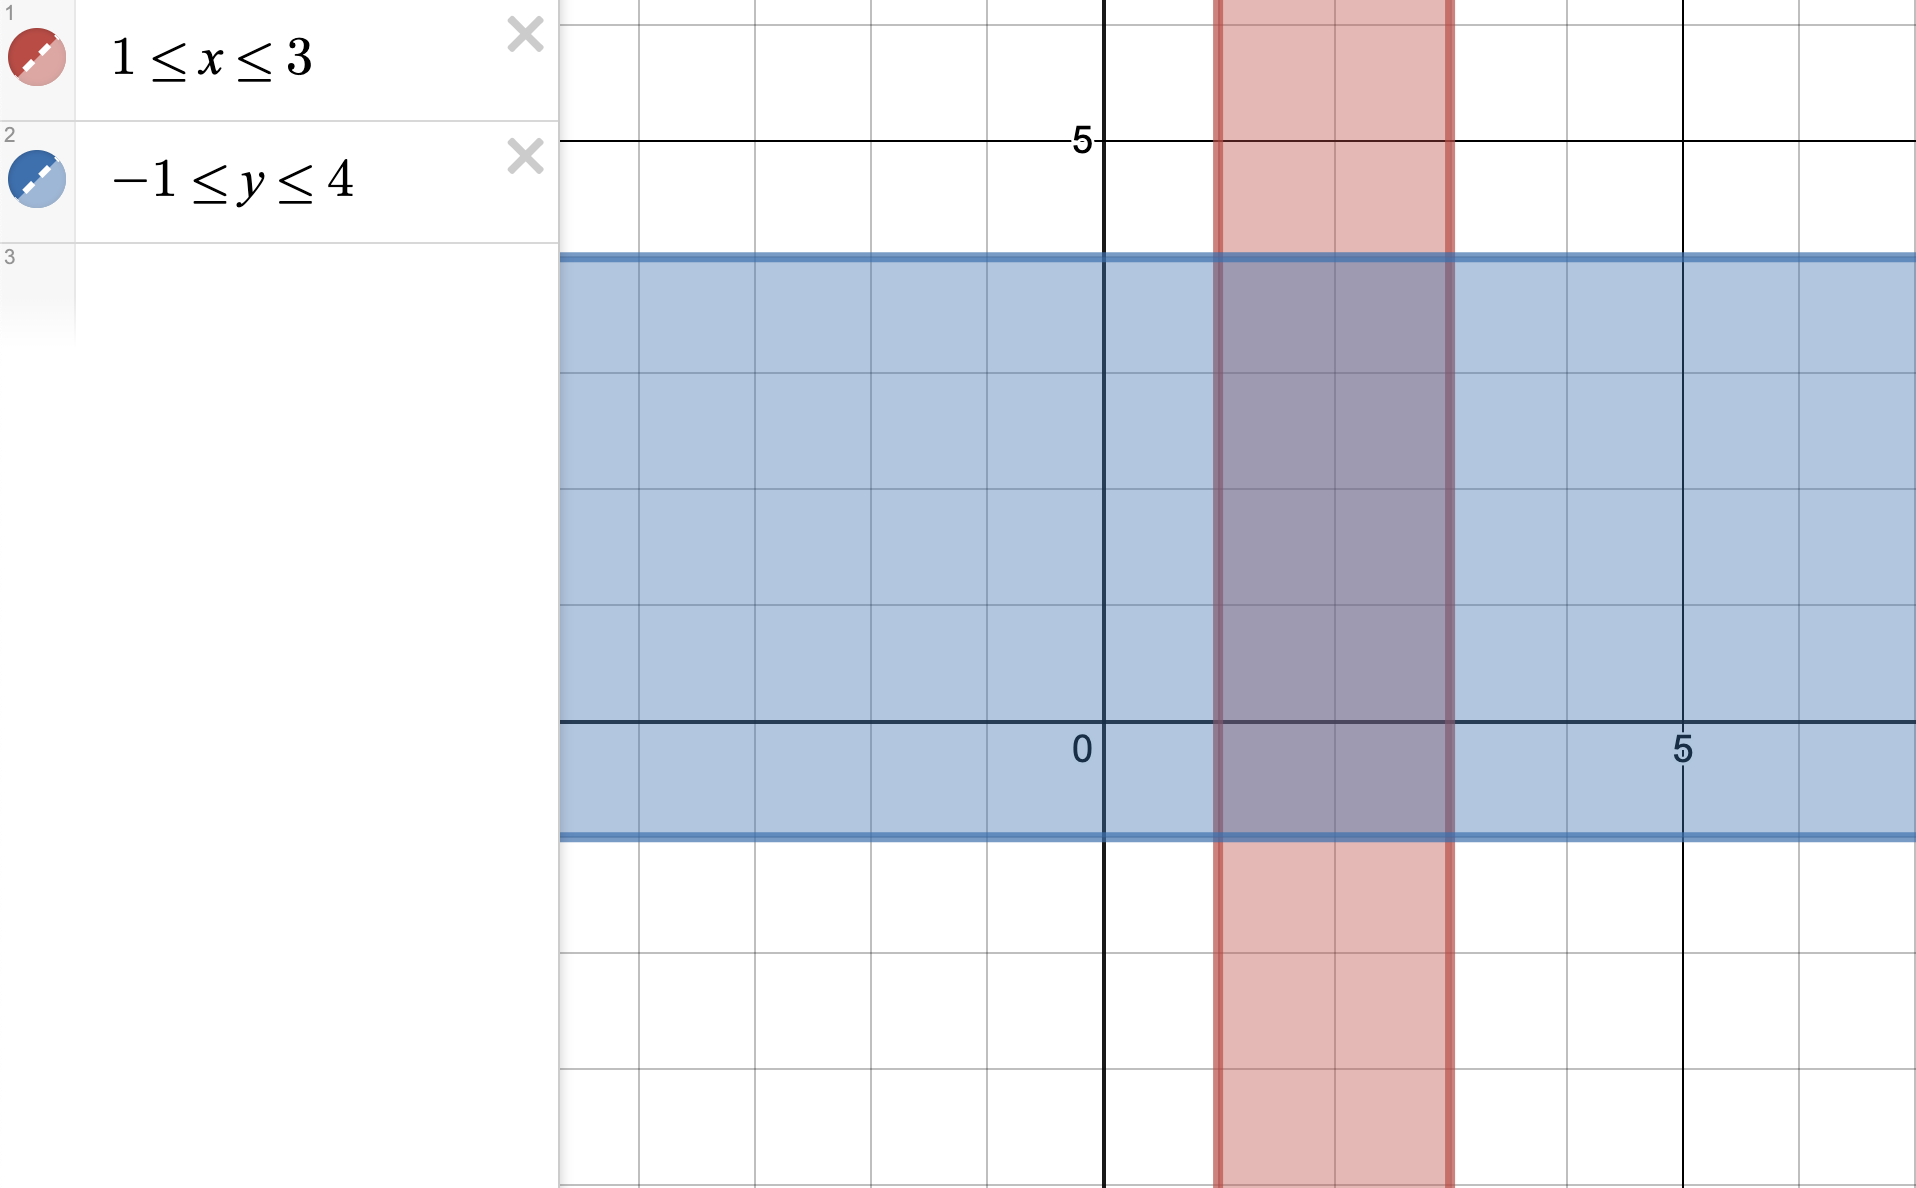
\includegraphics[width=\textwidth,height=\textheight,keepaspectratio]{bounding_box.png}
\end{frame}

\begin{frame}
\frametitle{Full System}
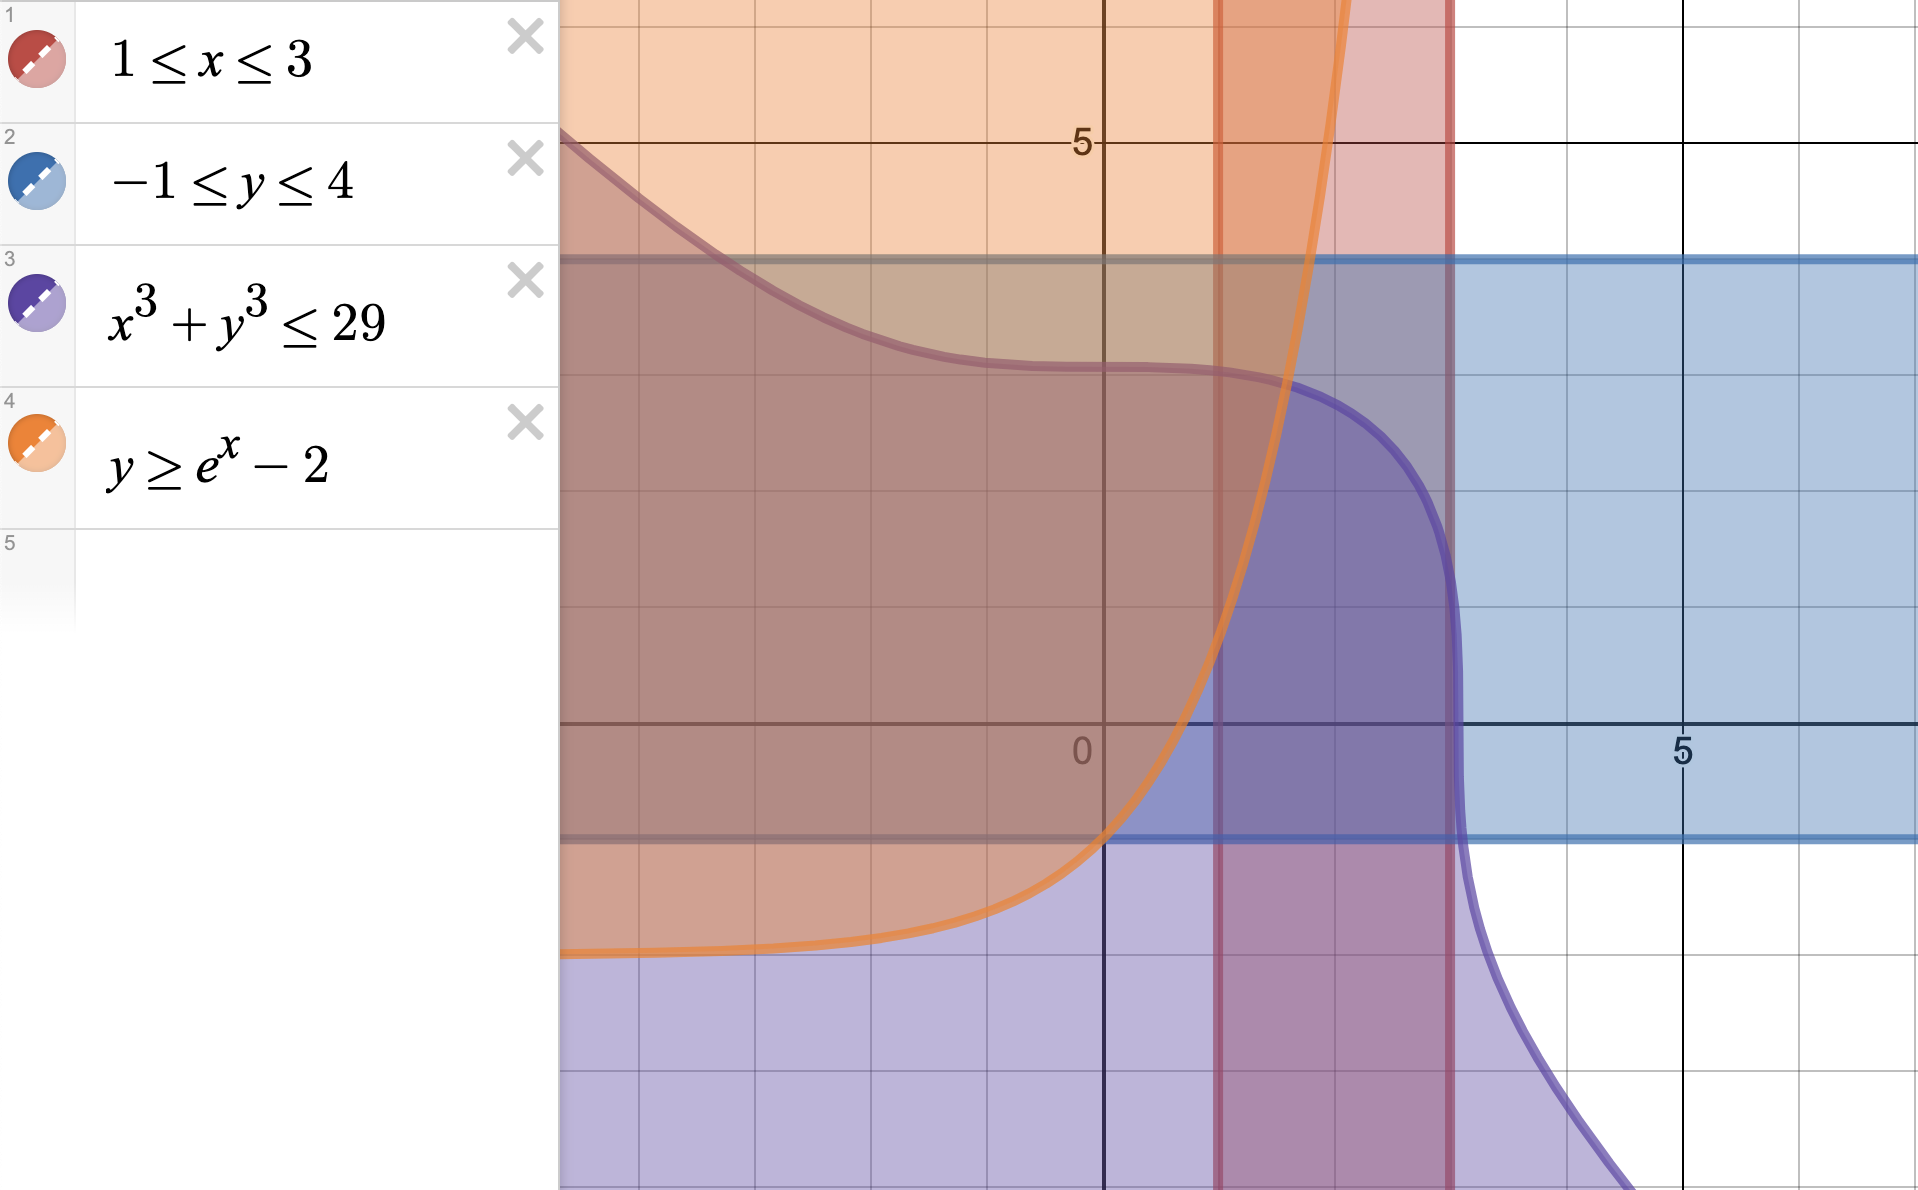
\includegraphics[width=\textwidth,height=\textheight,keepaspectratio]{full_system.png}
\end{frame}

\section{Tools}
\begin{frame}
\frametitle{Tools}
\begin{itemize}
  \item C
  \item C Math Library
  \item Intel Math Kernel Library (more specifically, the Vector Statistical Library)
  \item OpenMP
\end{itemize}
\end{frame}

\begin{frame}
\frametitle{Approach}
Generate a number in the rectangle and check if it satisfies.

Variables:
\end{frame}

\begin{frame}
\frametitle{Mathematical Solution}
I've used Maple to calcolate the following integral:
$$
\int_1^{a} (\sqrt[3]{29-x^3}-e^x+2)dx\approx 7.581218821150386e-01
$$
with $a=1.593743361313601$, point of intersection between the two curves defined by $y\ge e^x-2$ and $y\le \sqrt[3]{29-x^3}$.
\end{frame}

\begin{frame}
\frametitle{Error}
\end{frame}

\begin{frame}
\frametitle{Observations}
\end{frame}

\end{document}